

\documentclass[10pt]{beamer}

\mode<presentation>
{
 \usetheme{Boadilla}
\pagestyle{empty}

\setbeamerfont*{frametitle}{size=\normalsize,series=\bfseries}
\setbeamerfont*{block}{size=\normalsize,series=\bfseries}
%\setbeamertemplate{blocks}[rounded][shadow=true]
}


\usepackage[pdf]{pstricks}
\usepackage{pst-sigsys}


\definecolor{darkblue}{rgb}{0.0, 0.0, 0.40}
\setbeamercolor{title}{fg=darkblue}
\setbeamercolor{frametitle}{fg=darkblue}
\definecolor{darkgreen}{rgb}{0.0, 0.4, 0.0}

\usepackage{bbm}



\definecolor{links}{HTML}{2A1B81}
\hypersetup{colorlinks,linkcolor=,urlcolor=links}

\newcommand{\fs}[2]{#2}

\title[]{Systems and Circuits}
\author[\textcolor{blue}{Systems and Circuits}]{\textcolor{darkblue}{Pablo M. Olmos} (olmos@tsc.uc3m.es)\\ \textcolor{darkblue}{Emilio Parrado} (emipar@tsc.uc3m.es)}
\institute{\textcolor{white}{UC3M}}


\AtBeginSection[]
{
  \begin{frame}<beamer>{Index}
    \tableofcontents[currentsection,currentsubsection]
  \end{frame}
}

\begin{document}
\frame{
\titlepage
\thispagestyle{empty}
\begin{center}

\includegraphics[scale=0.05]{Figures/logouc3m.pdf}
\end{center}
}





\frame{
\frametitle{Systems and Circuits $\rightarrow$ Introduction to Electrical Engineering}

\begin{itemize}
\item Introduce the basic concepts of signals and systems.
\end{itemize}

\begin{columns}[T]
\begin{column}{0.4\textwidth}
\centering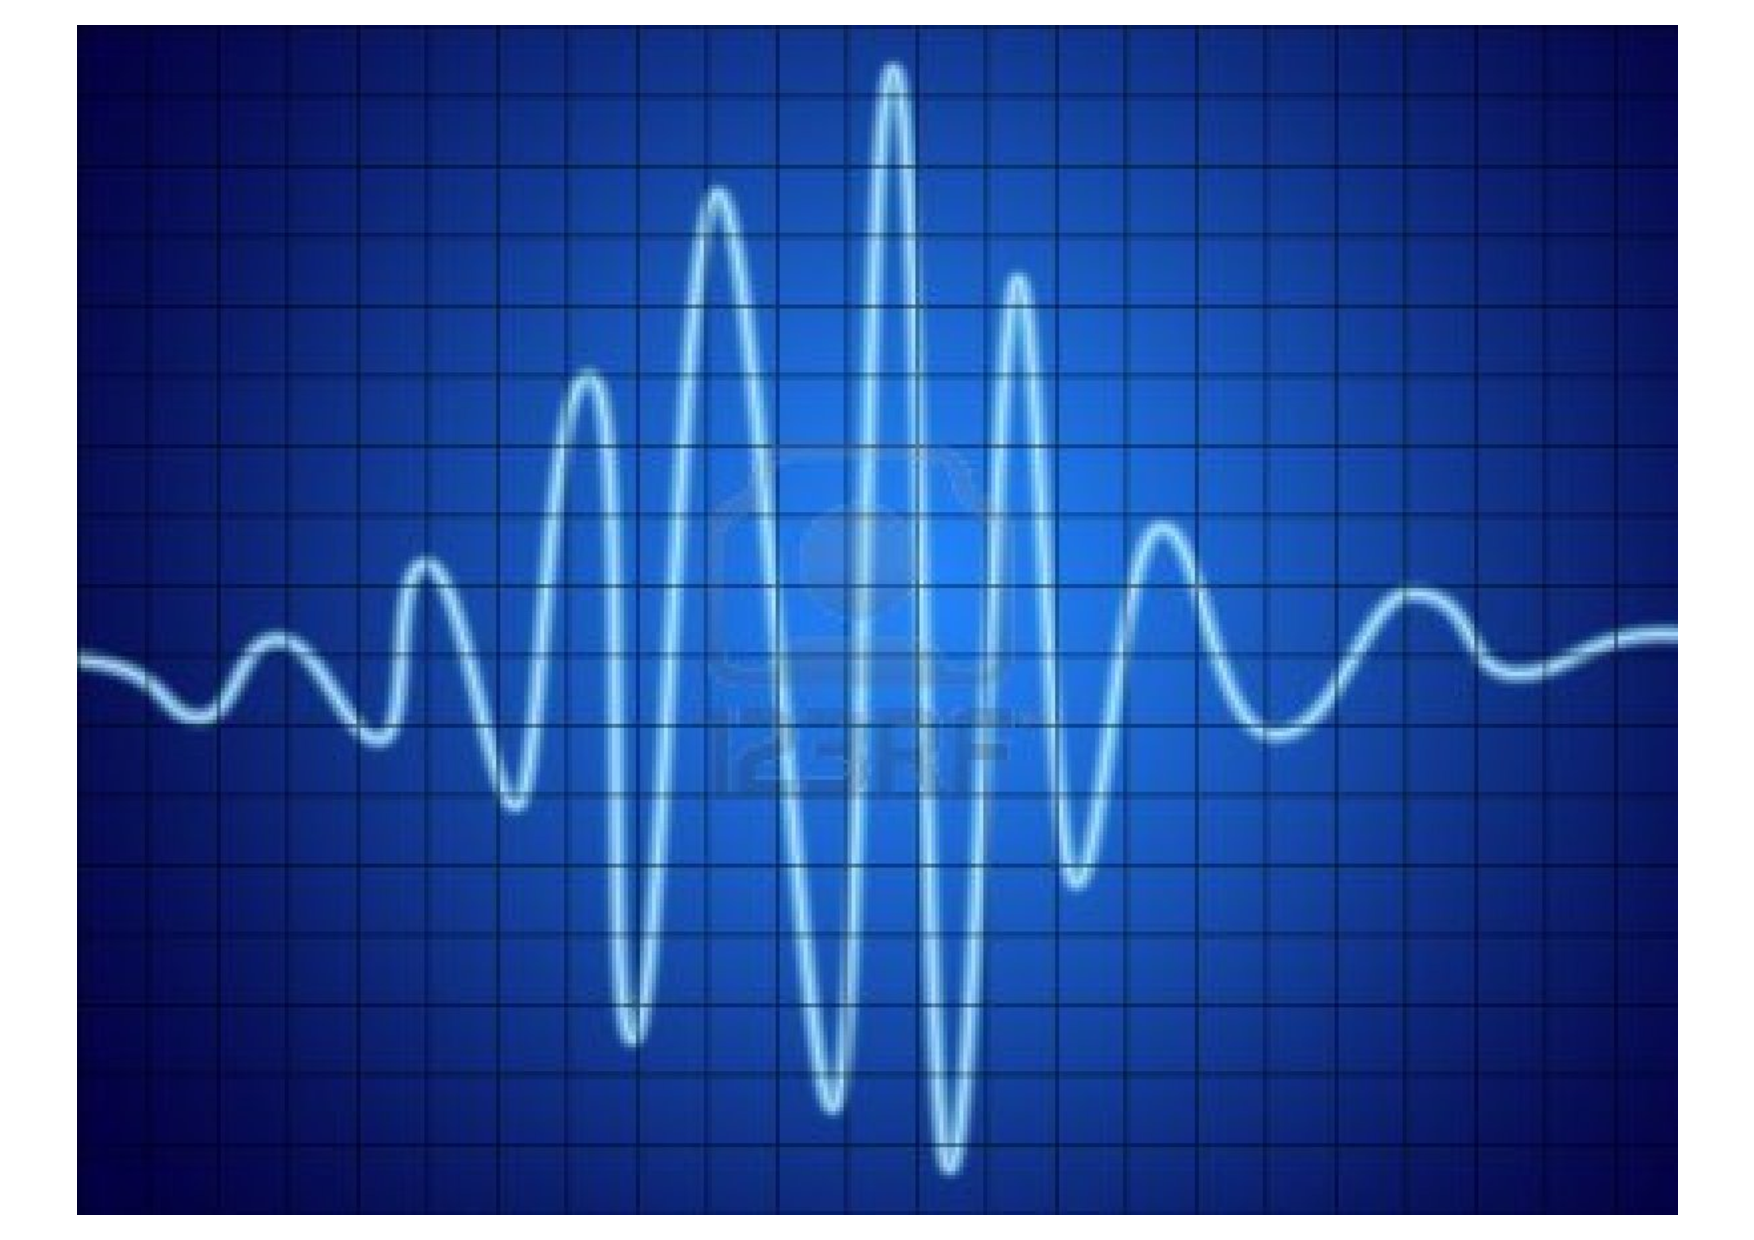
\includegraphics[width=4cm,height=2cm]{Figures/Signal1.pdf}
\end{column}
\begin{column}{0.4\textwidth}
\centering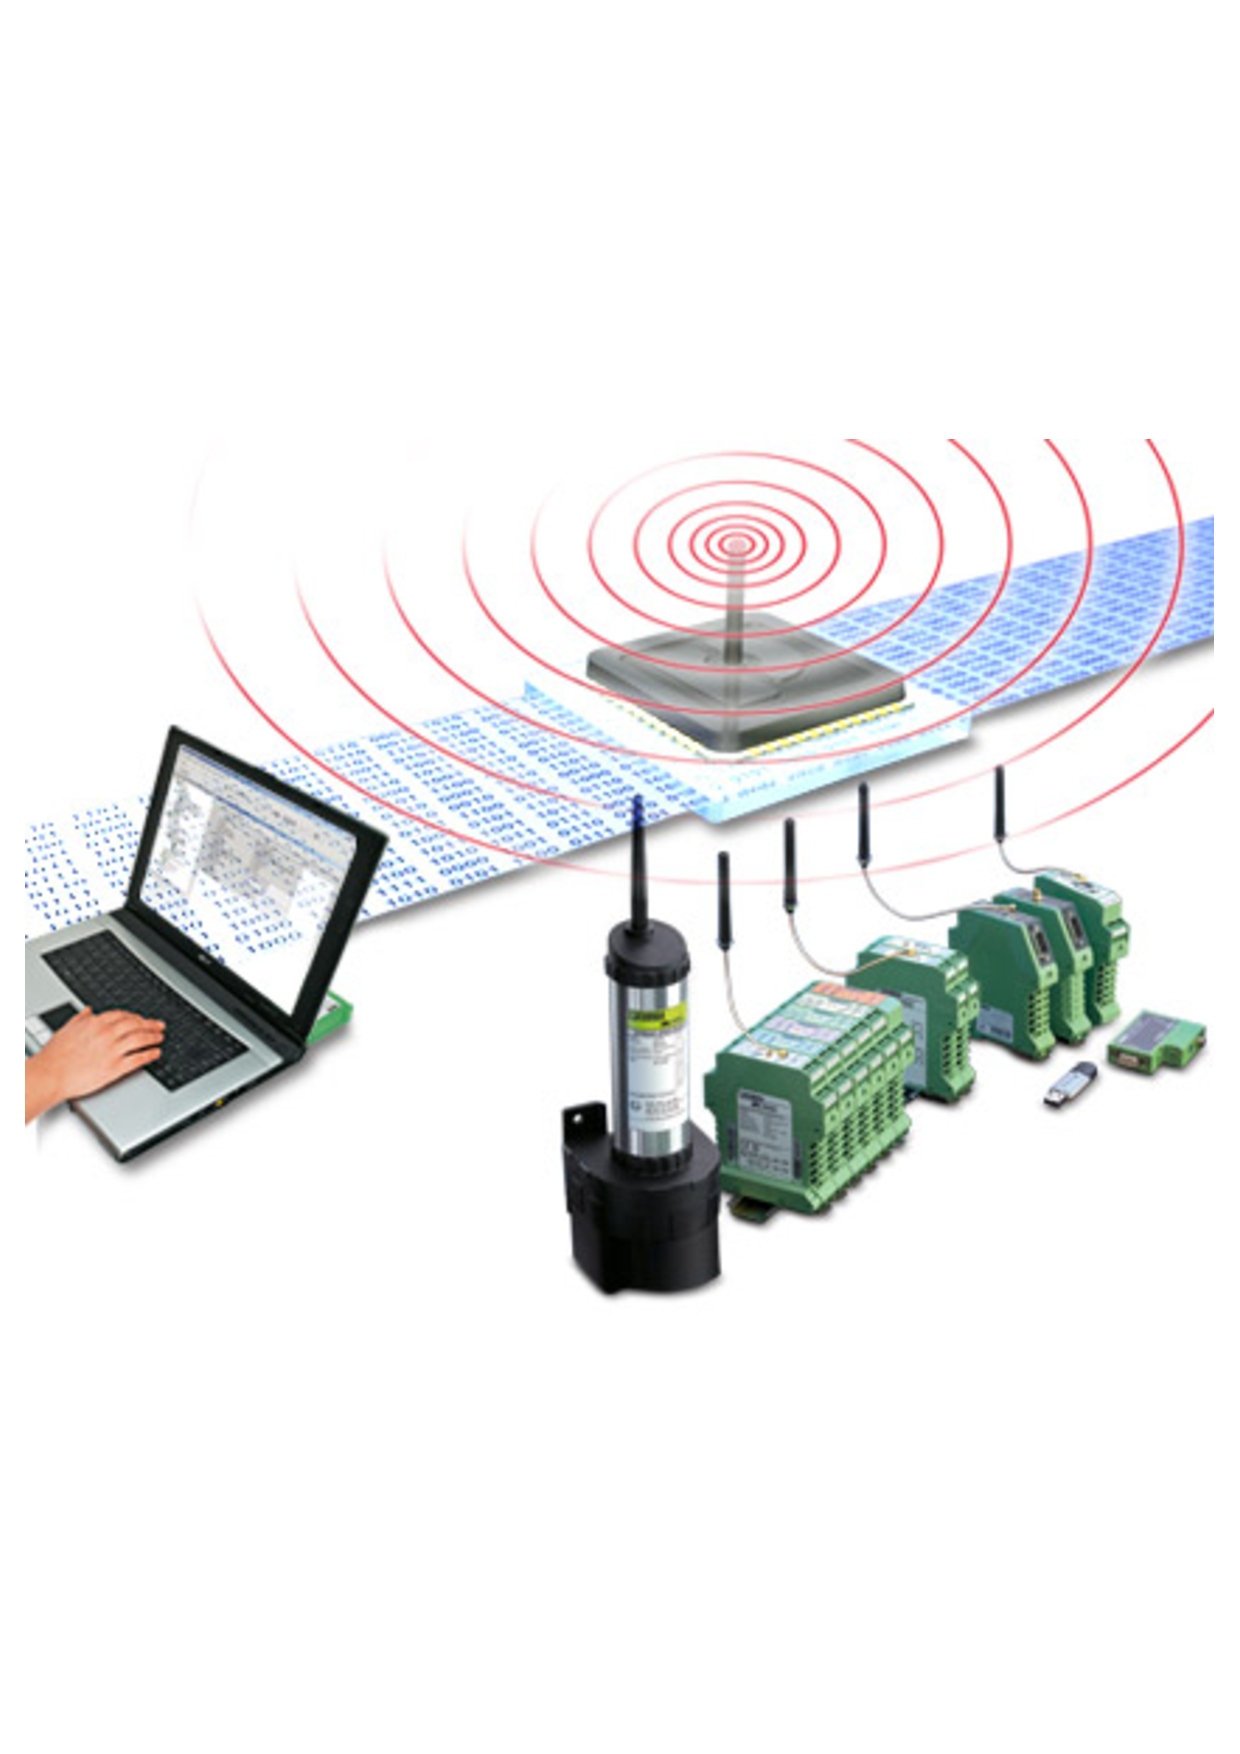
\includegraphics[width=2cm,height=2cm]{Figures/Signal2.pdf}
\end{column}
\end{columns}

%\begin{figure}[h]
%\centering
%\begin{tabular}{cc}
%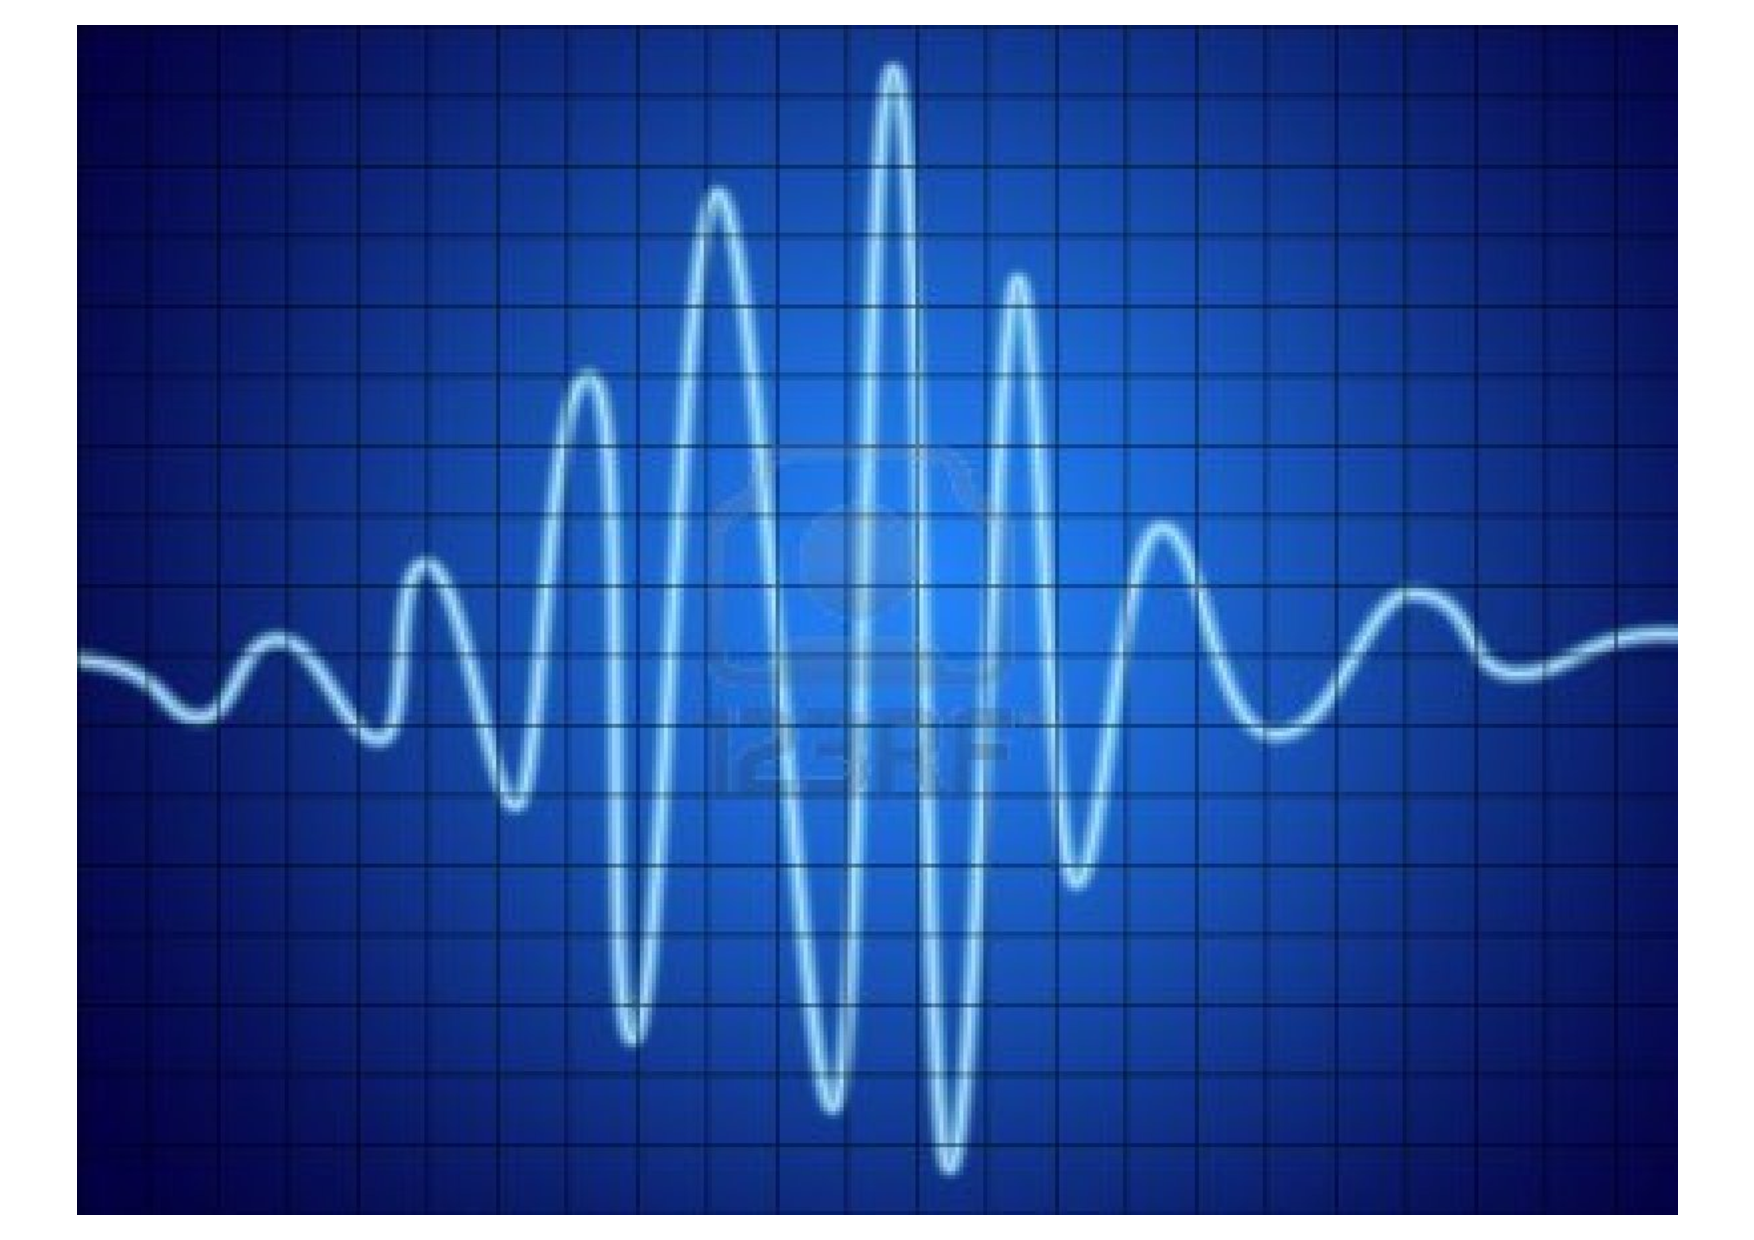
\includegraphics[width=4 cm,height=2cm]{Figures/Signal1.pdf} & 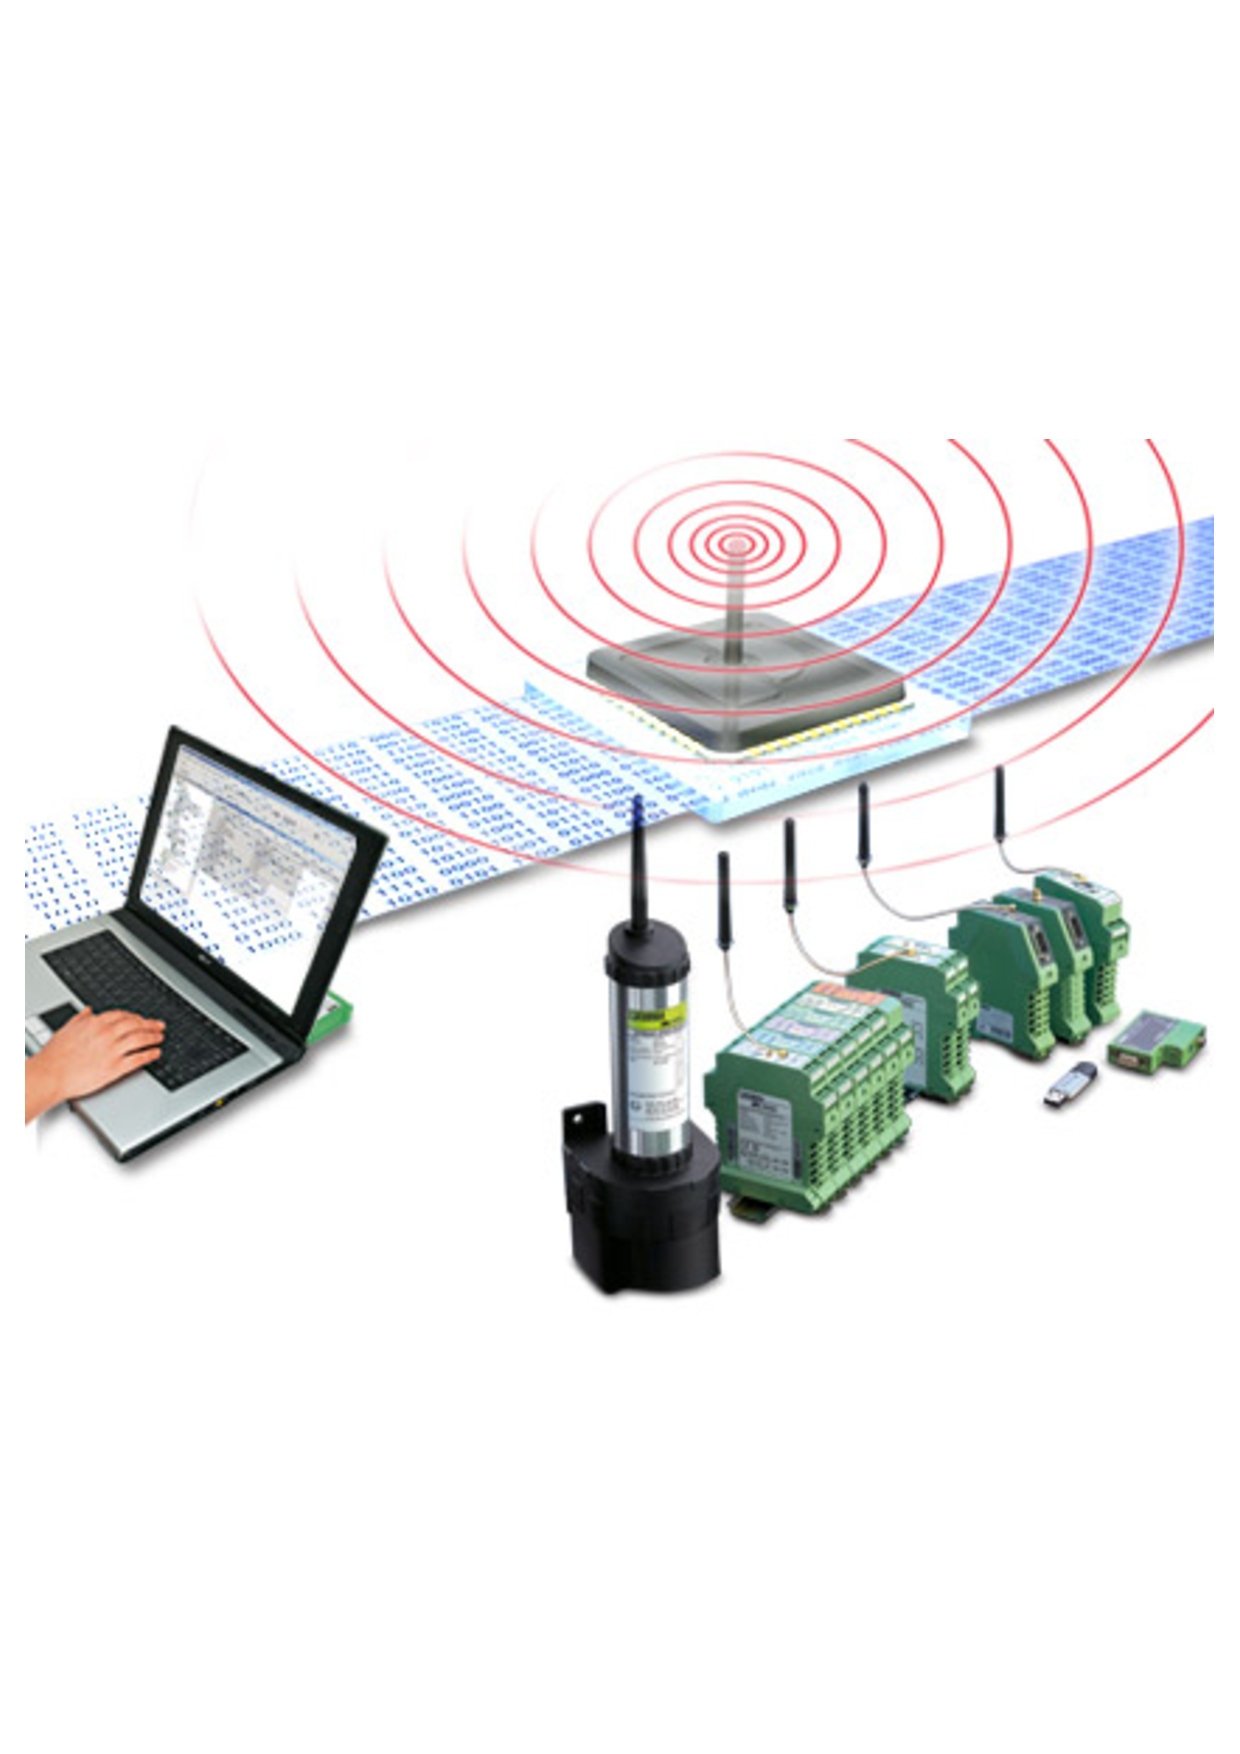
\includegraphics[width=4 cm,height=4cm]{Figures/Signal2.pdf}
%\end{tabular}
%\end{figure}




\begin{itemize}
\item Introduce the basic concepts of electric circuit analysis.
\end{itemize}

\begin{columns}[T]
\begin{column}{0.4\textwidth}
\centering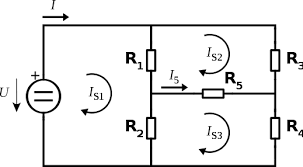
\includegraphics[scale=0.5]{Figures/Plot1.png}
\end{column}
\begin{column}{0.4\textwidth}
\centering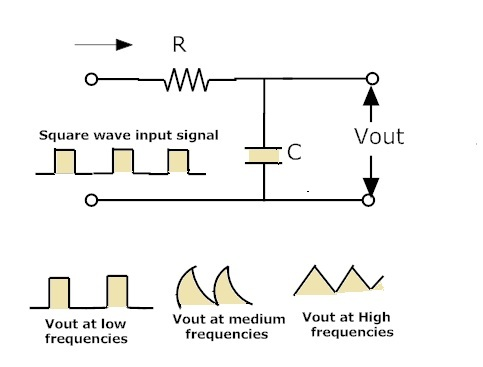
\includegraphics[scale=0.5]{Figures/Plot2.jpeg}
\end{column}
\end{columns}

}



\frame{
\frametitle{Course materials}
\underline{1.- Basic books:} (I really encourage you to follow them!)
\begin{itemize}
\item Signals and systems. Alan V. Oppenheim.
\item Electric circuits  6th ed. James William Nilsson.
\end{itemize}

\begin{columns}[T]
\begin{column}{0.4\textwidth}
\centering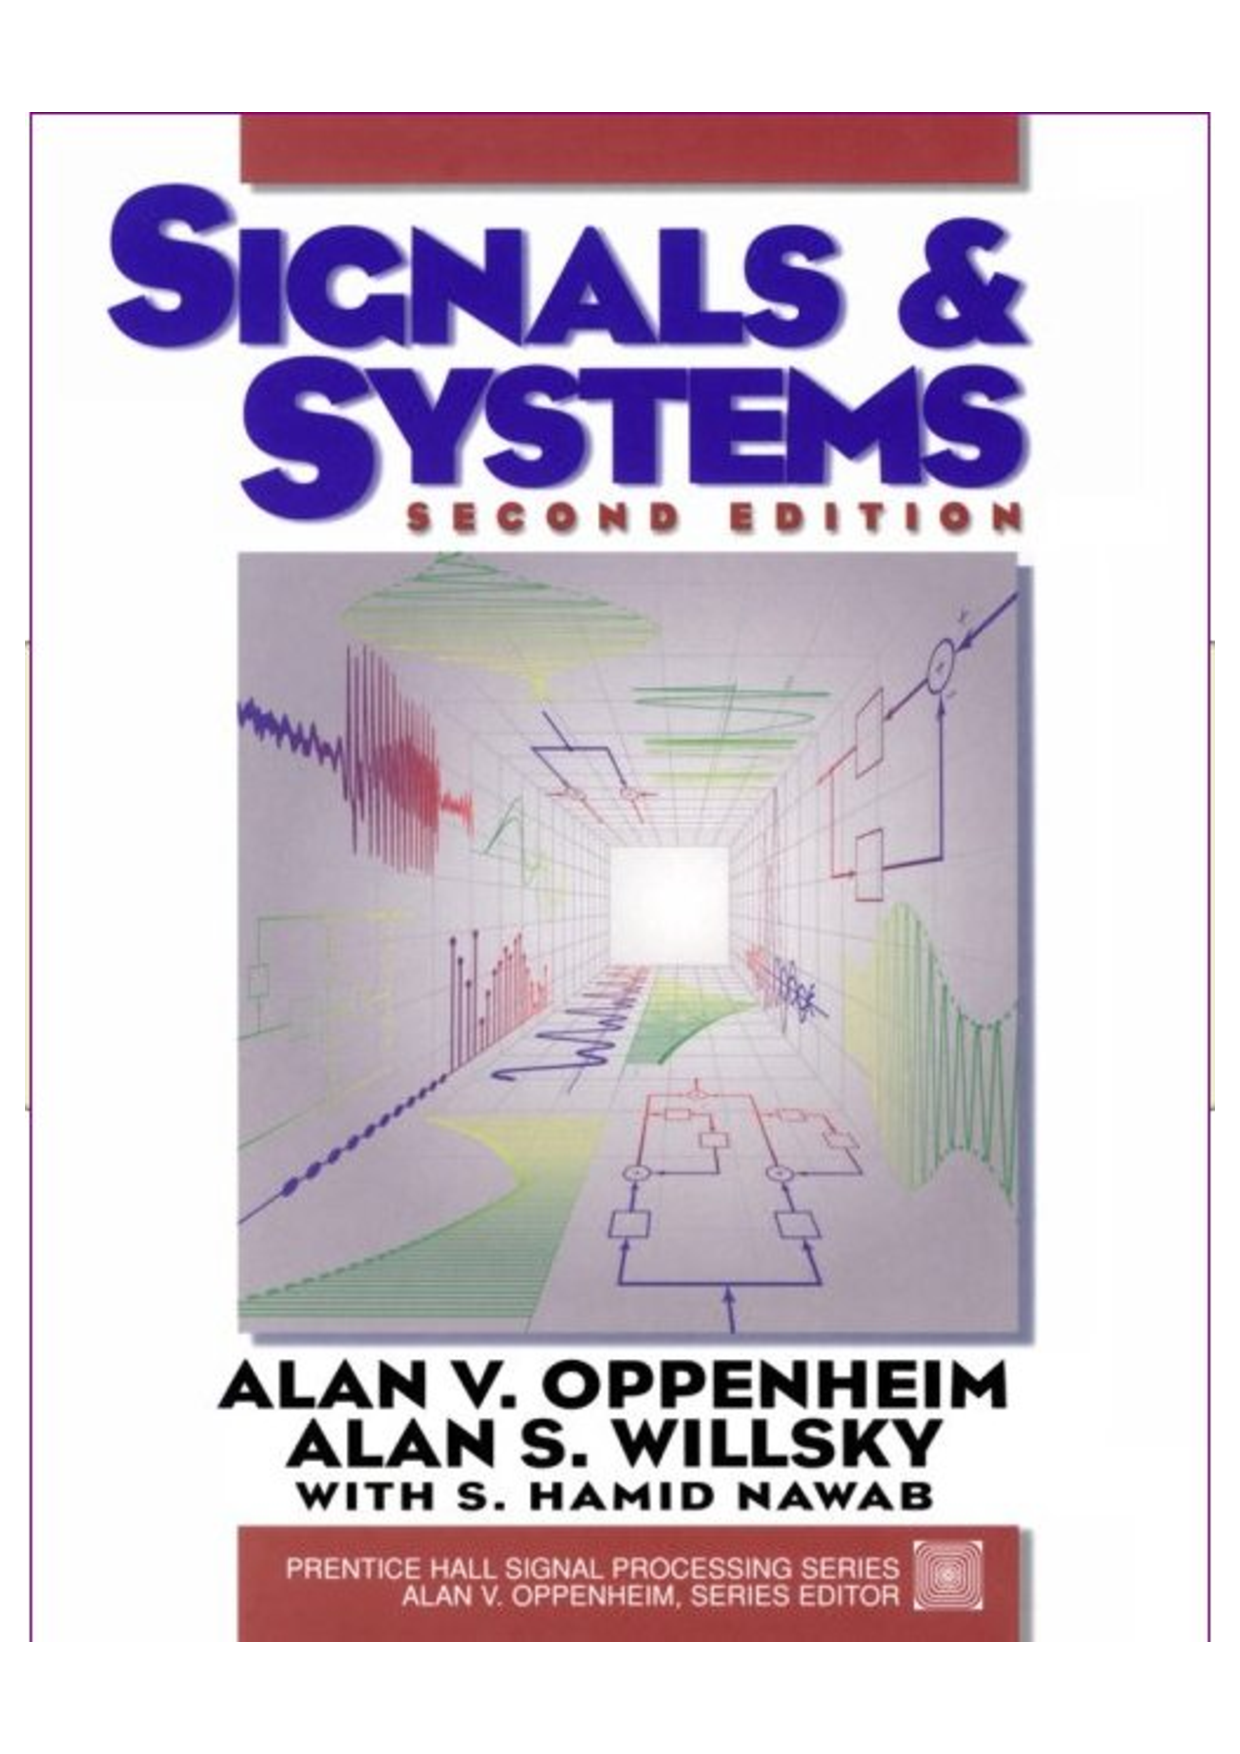
\includegraphics[scale=0.15]{Figures/Signal6.pdf}
\end{column}
\begin{column}{0.4\textwidth}
\centering
\includegraphics[scale=0.15]{Figures/Signal7.pdf}
\end{column}
\end{columns}
}

\frame{
\underline{2.- Slides that I will  use in class} 
\begin{itemize}
\item Aula Global. 
\item Please report mistakes you find (typos, errors in formulas, etc...). Thank you very much!!
\end{itemize}
\underline{3.- Online material } 
\begin{itemize}
\item Large amount of resources at your disposal. Just an example...
\begin{itemize}
\item M.I.T. Open courseware $\Rightarrow$ Signal and Systems.  \\
\url{http://ocw.mit.edu/resources/res-6-007-signals-and-systems-spring-2011/index.htm}
\item M.I.T. Open courseware $\Rightarrow$ Circuits and Electronics.  \\
\url{http://ocw.mit.edu/courses/electrical-engineering-and-computer-science/6-002-circuits-and-electronics-spring-2007/index.htm}
\end{itemize}
\end{itemize}
}



\section{Introduction to Signal Processing}


\frame{
\frametitle{Signal Processing}

\begin{itemize}
\item The concepts of signal and systems arise in an extremely wide variety of fields.
\begin{itemize}
\item Communications
\item Aeronautics
\item Circuit design
\item Acoustics
\item Biomedical engineering
\item Energy generation
\item Speech Processing
\item Machine Learning
\item Computer Vision 
\item ...
\end{itemize} 
\end{itemize}

\begin{alertblock}{}
Signal processing is a cornerstone of any engineering branch. You will apply the concepts and tools acquired in this course for the next four years.
\end{alertblock}

}


\frame{
\frametitle{The physical world: representation by means of signals and systems}
\begin{itemize}
\item Signals: Functions that represent variations in physical magnitudes.
\item Information is contained in the variation with respect some independent variables.
\end{itemize}
\begin{figure}
\centering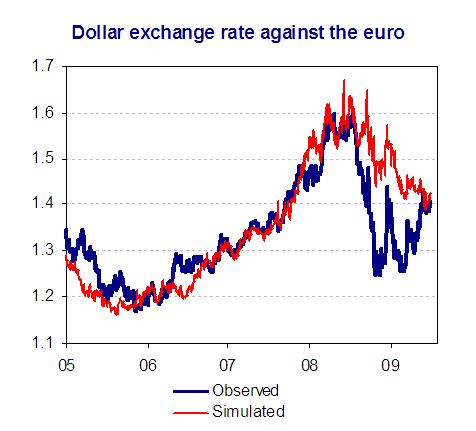
\includegraphics[scale=0.55]{Figures/Plot5.jpeg}
\caption{\small{Source \url{http://voxeu.org/article/euro-dollar-exchange-rate-during-crisis}. }}
\end{figure}
}

%\frame{
%\frametitle{The physical world: representation by means of signals and systems}
%\begin{itemize}
%\item Signals: Functions that represent variations in physical magnitudes.
%\item Information is contained in the variation with respect some independent variables.
%\end{itemize}
%\begin{figure}
%\centering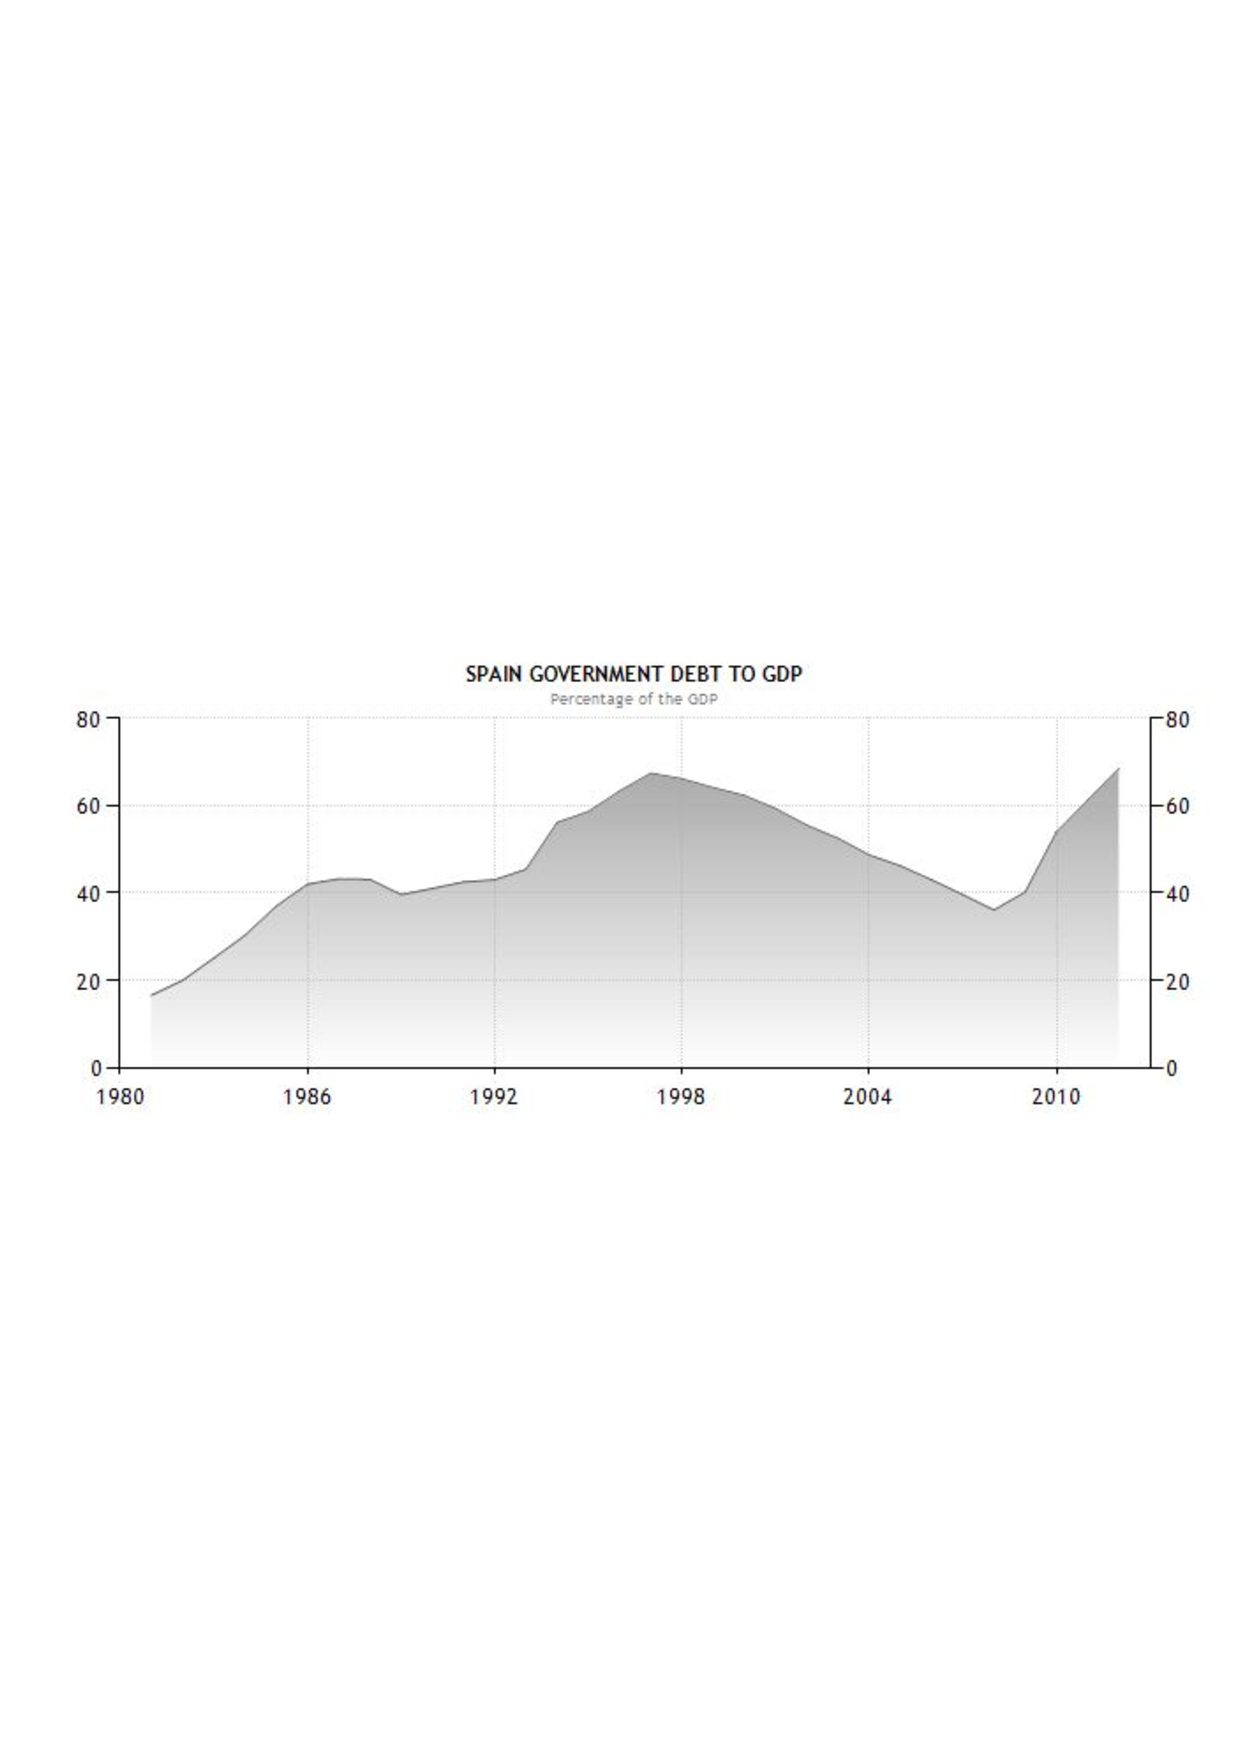
\includegraphics[scale=0.4]{Figures/Signal8.pdf}
%\caption{Spanish debt evolution along the time (GDP: gross domestic product). }
%\end{figure}
%}


\frame{
\frametitle{Example of signals: electromagnetic wave}
\begin{figure}
\centering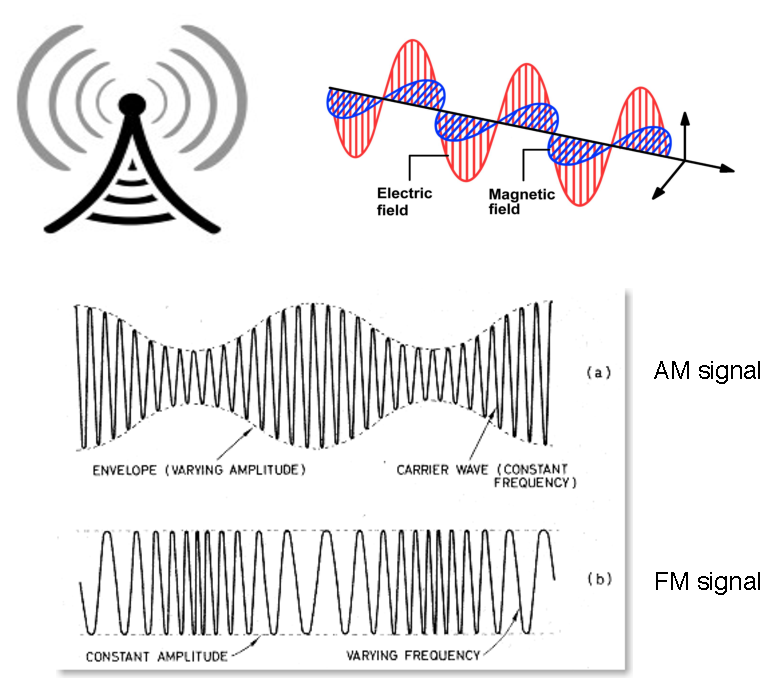
\includegraphics[scale=0.7]{Figures/Signal10.pdf}
%\caption{Spanish debt evolution along the time (GDP: gross domestic product). }
\end{figure}
}

\frame{
\frametitle{Example of signals: digital image}
\begin{figure}
\centering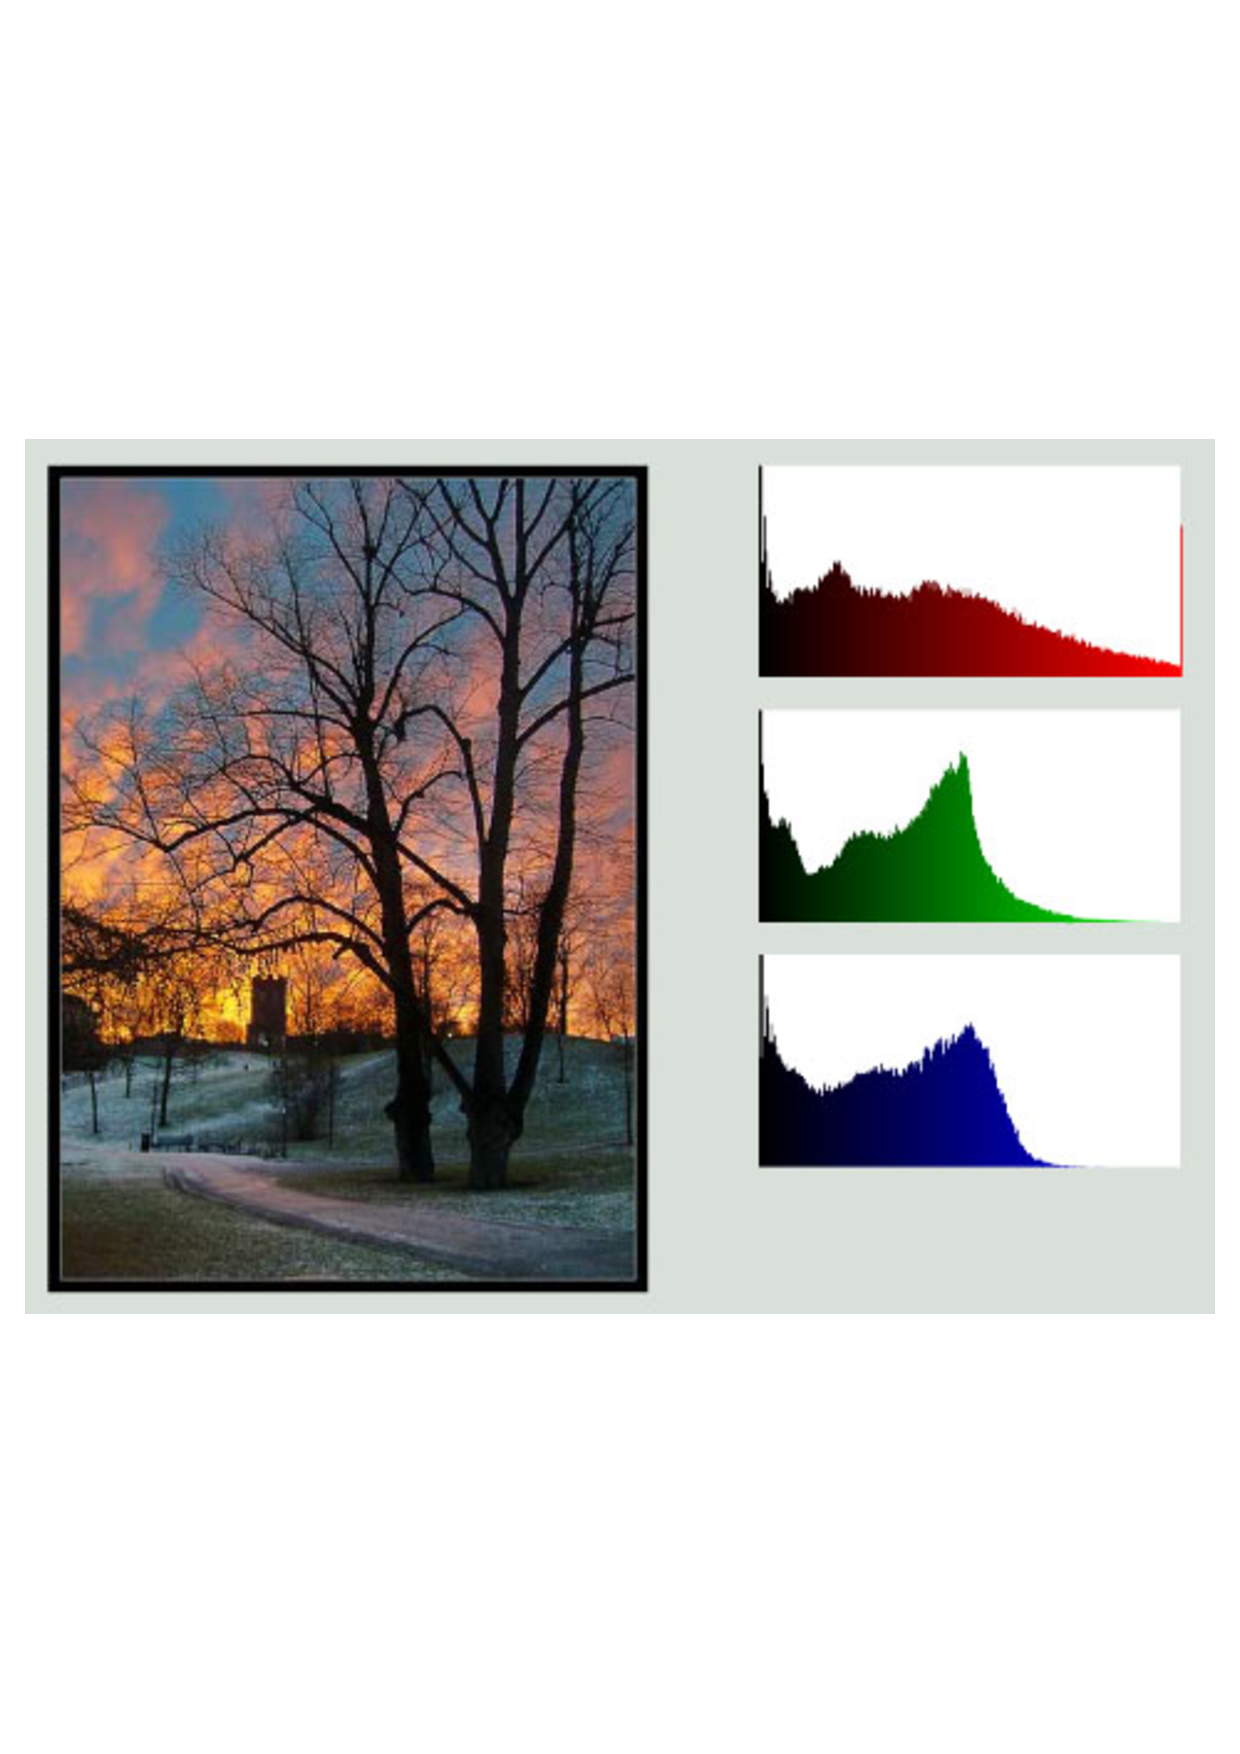
\includegraphics[scale=0.4]{Figures/Signal12.pdf}
\caption{RGB level per pixel. }
\end{figure}
}

\frame{
\frametitle{Example of signals: Electrocardiogram (ECG) signal}
\begin{figure}
\centering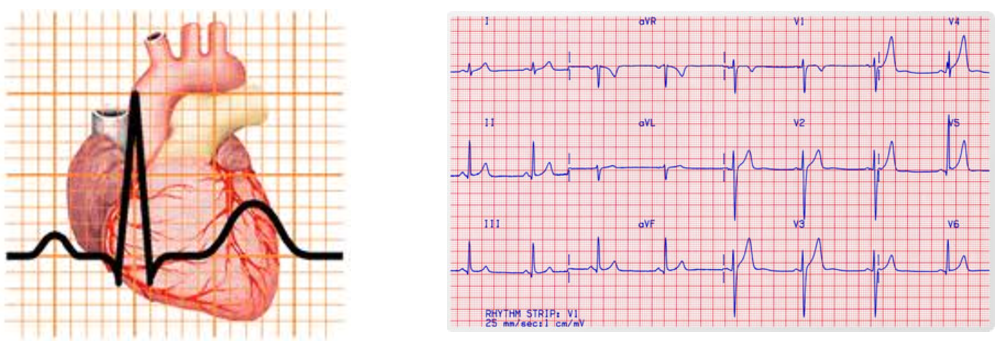
\includegraphics[scale=0.7]{Figures/Signal15.pdf}
\end{figure}

\begin{block}{}
Electrical activity of the heart over a period of time: The ECG device detects and amplifies the tiny electrical changes on the skin that are caused when the heart muscle depolarizes during each heartbeat.
\end{block}
}

\frame{

\frametitle{Systems}
\begin{itemize}
\item Physical device that performs an operation on a signal.
\item Any process that transforms one signal into another.
\item Systems can model the behavior of a chemical process, a hydraulic system, an electric circuit, a communication channel, ...
\end{itemize}

\begin{exampleblock}{Signal Processing}
Area of systems engineering, electrical engineering and applied mathematics that deals with the  analysis of the properties of signals and the design of systems that attain an specific purpose.
\end{exampleblock}

}



\frame{
\frametitle{System examples: electric circuits}
\begin{figure}
\centering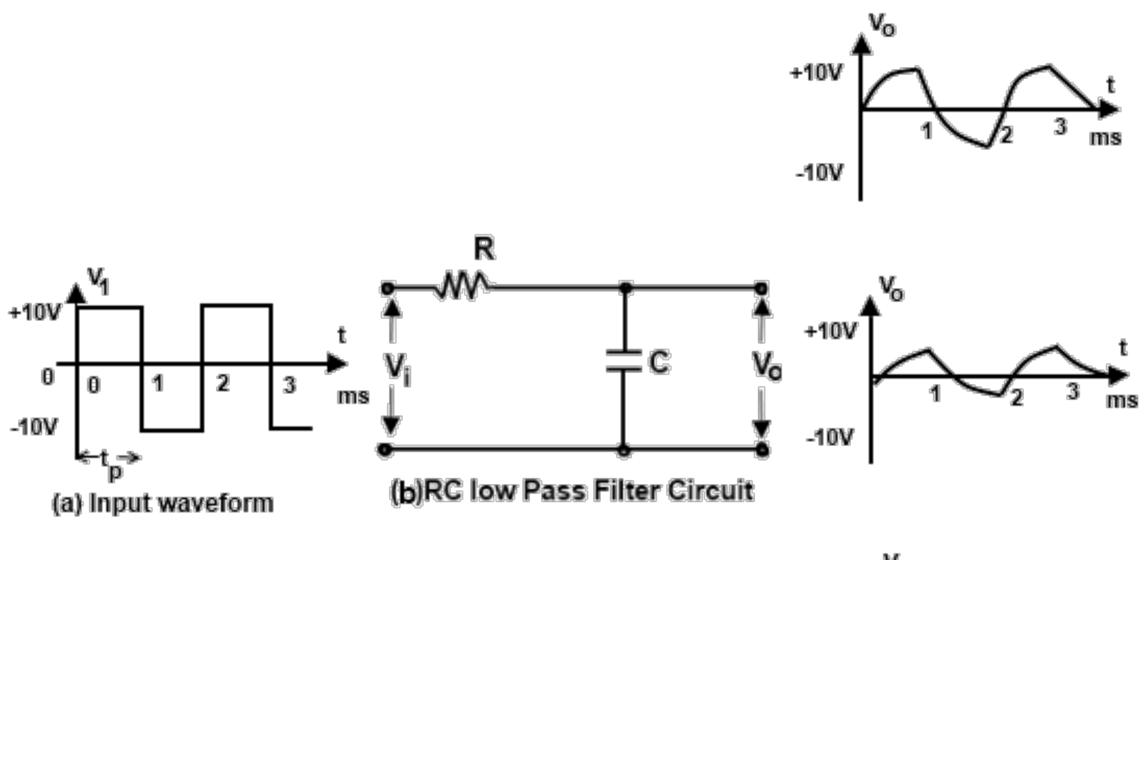
\includegraphics[scale=0.5]{Figures/Signal29.pdf}
\end{figure}
In this course, we will apply what we have learnt about signal and systems to analyze elementary electric circuits.
}

\frame{

\begin{figure}
\centering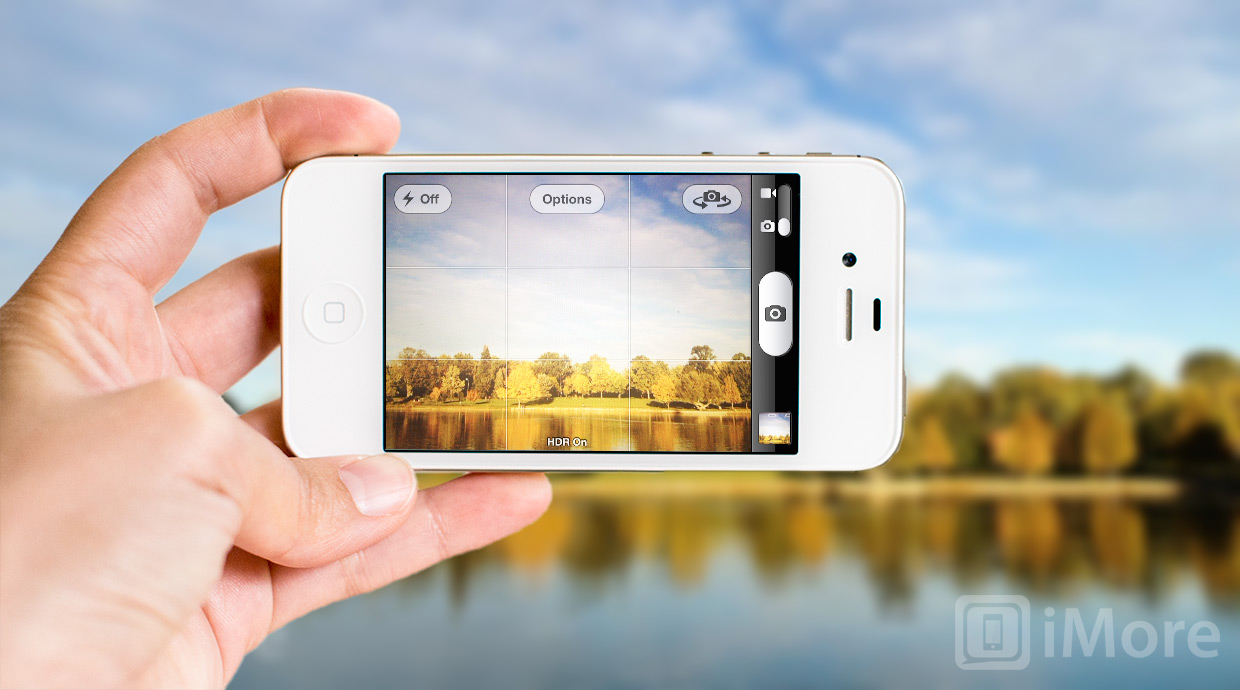
\includegraphics[scale=0.15]{Figures/iphone1.jpg}
%\caption{Voice (pressure) signal $\Rightarrow$ Voltage signal}
\end{figure}
\begin{figure}
\centering
\includegraphics[scale=0.15]{Figures/iphone2.jpg}
%\caption{Voice (pressure) signal $\Rightarrow$ Voltage signal}
\end{figure}

}


\frame{

\begin{itemize}
\item Information (picture) is originally encoded in a signal by means of signal intensity at different frequencies (colors).
\item A light sensor is composed by a grid of millions of little squares (pixels), each one kind of like a solar cell
\begin{itemize}
\item Depending on the light intensity at a particular color (frequency), they generate an electrical signal.
\begin{align*}
v[n,f]=p(I[n,f]) 
\end{align*}
\item $I[f,n]$ is the light intensity at frequency $f$ rad/s at the $n$-pixel. Imagine we only consider three frequencies (colors): red, blue, green (RGB).
\item $v[n,f]$  is the voltage at the output of the $n$-pixel at frequency $f$.
\end{itemize}
\end{itemize}

\begin{figure}
\centering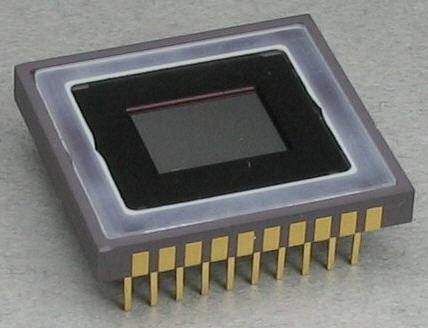
\includegraphics[scale=0.5]{Figures/CCD_Image_sensor.jpg}
%\caption{Voice (pressure) signal $\Rightarrow$ Voltage signal}
\end{figure}

}


\frame{
\begin{itemize}
\item The signal $v[n,f]$ typically can take any real value in a certain range $[0,V]$.
\item Digital electronics only allow a discrete number of levels. E.g. 256 levels per frequency are encoded in $8$ bits ($2^8=256$).
\item \textbf{Quantization}
\end{itemize}

\begin{figure}
\centering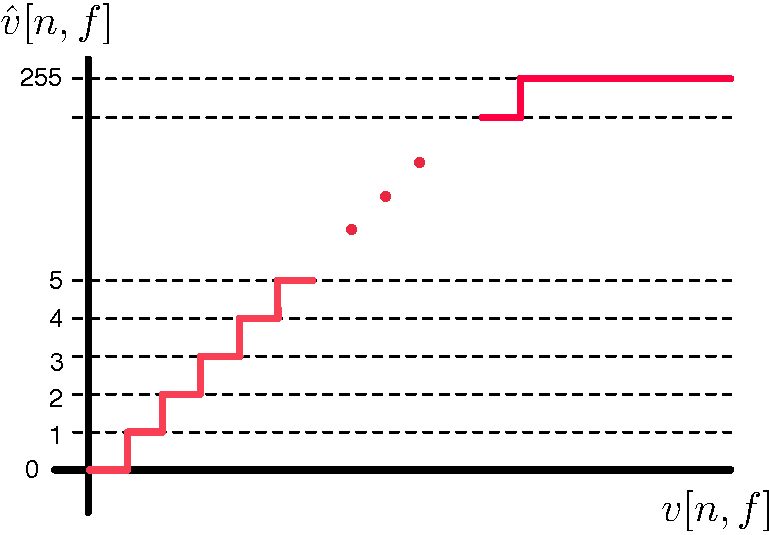
\includegraphics[scale=0.5]{Figures/quantizer.pdf}
%\caption{Voice (pressure) signal $\Rightarrow$ Voltage signal}
\end{figure}


}

\frame{
\begin{itemize}
\item Imagine $256$ color level and three frequencies (red, green, blue).
\item Each quantized pixel $\hat{v}[n,f]$ needs $3\times 8$ bits$=3$ bytes.
\item Imagine the camera has $5$ megapixels.
\item Each image requires a memory of $5\times 10^6 \times 3 \approx 15$ MB.
\item However the image file finally stored in the hard disk (jpg file) has a weight of only $0.5$ MB.
\item The \textbf{image has been compressed}.
\end{itemize}




\begin{block}{}
The objective of image compression is to reduce irrelevance and redundancy of the image data in order to be able to store or transmit data in an efficient form.
\end{block}

\begin{figure}
\centering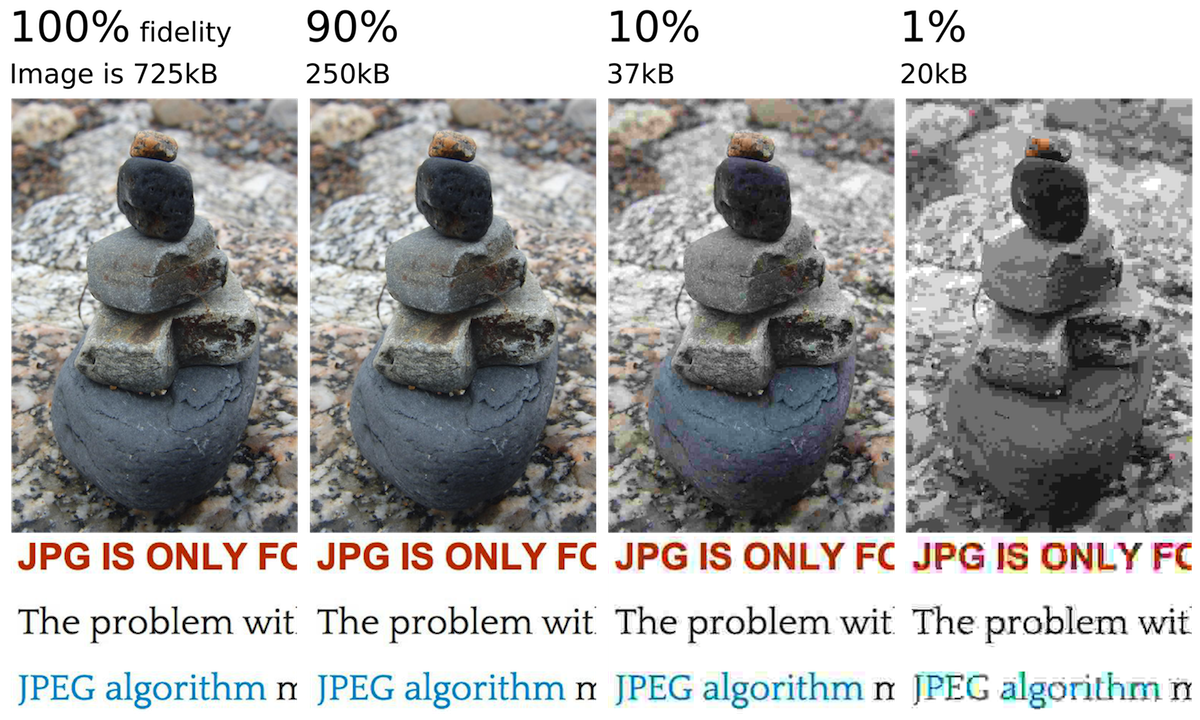
\includegraphics[scale=0.3]{Figures/Plot6.png}
\caption{\small{Source: \url{https://sites.google.com/site/keremitgsnotes/chapter-6/compression}}}
\end{figure}

%\begin{center}
%\begin{pspicture}[](6,2)
%   \pssignal(-1.75,1){x}{$\hat{v}[n,f]$}
%   \pssignal(-1.75,0){n}{$n=1,\ldots,5 \times 10^6$}
%   \psblock(1.5,1){a}{Image Compressor}
%   %\psblock(4,1){b}{$h[n], H(z)$}
%   \pssignal(4.75,1){y}{$c[u,f]$}
%   \pssignal(4.75,0){c}{$u=1, \ldots, d$}
%   \pssignal(4.75,-1){d}{$d<<5 \times 10^6$}
%   %-----------------
%   \psset{arrows=->}
%   \ncline{x}{a}  \ncline{a}{y}  %\ncline{b}{y}
%\end{pspicture}
%\end{center}



}

\frame{
\begin{itemize}
\item Bits are encoded in a electromagnetic signal for transmission.
\item We create an electric current signal $i(t)$  over an antenna, which creates a electromagnetic field $e(t)$ of similar properties (amplitude, frequency, ...).
\end{itemize}


\begin{figure}
\centering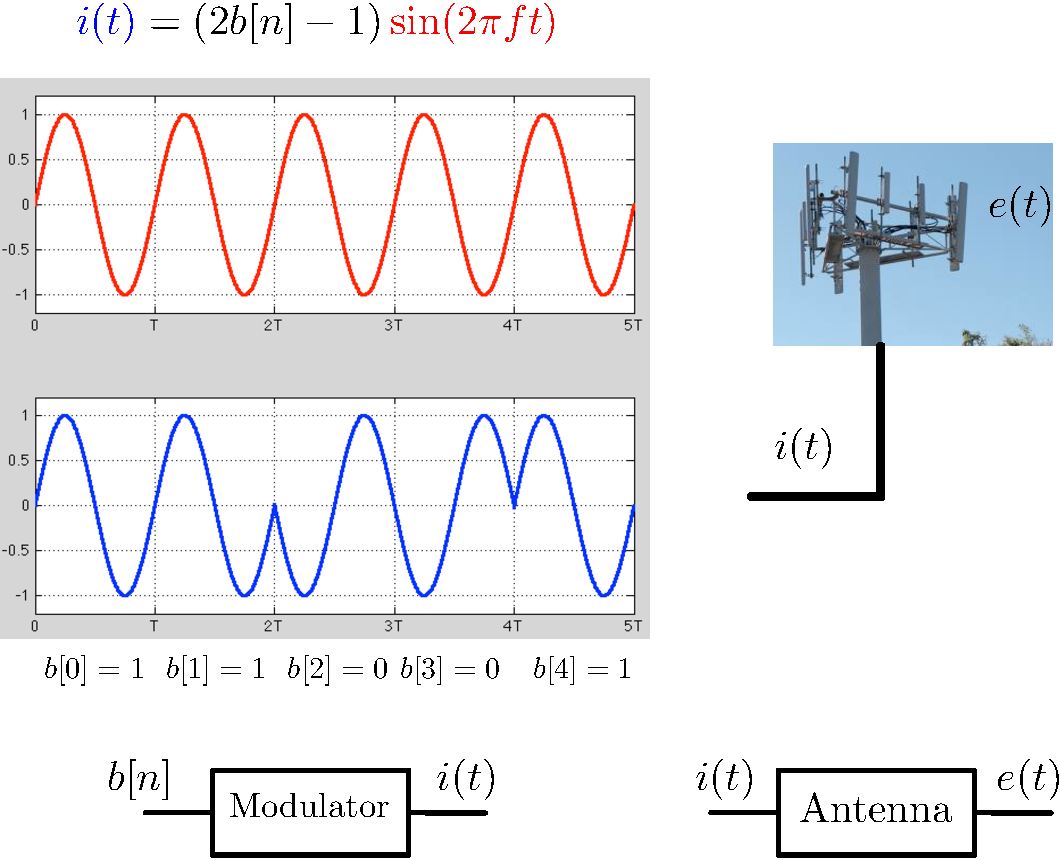
\includegraphics[scale=0.5]{Figures/antenna.pdf}
%\caption{Voice (pressure) signal $\Rightarrow$ Voltage signal}
\end{figure}

}



\frame{
\frametitle{To sum up}
\begin{itemize}
\item The notions of signal and systems are extremely general concepts.
\item Range of applications and problems is huge.
\end{itemize}

Where should we start?

\begin{block}{}
An important and fundamental notion in dealing with signals and systems is that by carefully choosing subclasses of each with particular properties that can then be exploited, we can analyze and characterize complex signals and systems in great depth.\\
\emph{Alan Oppenheim}
\end{block}

In other words, we will start with basic definitions and concepts to understand and design complex systems.

}

\frame{

\begin{exampleblock}{}
\textbf{MATHEMATICAL FRAMEWORK}+\textbf{BASIC BUILDING BLOCKS}
\end{exampleblock}

\begin{tabular}{cc}
\centering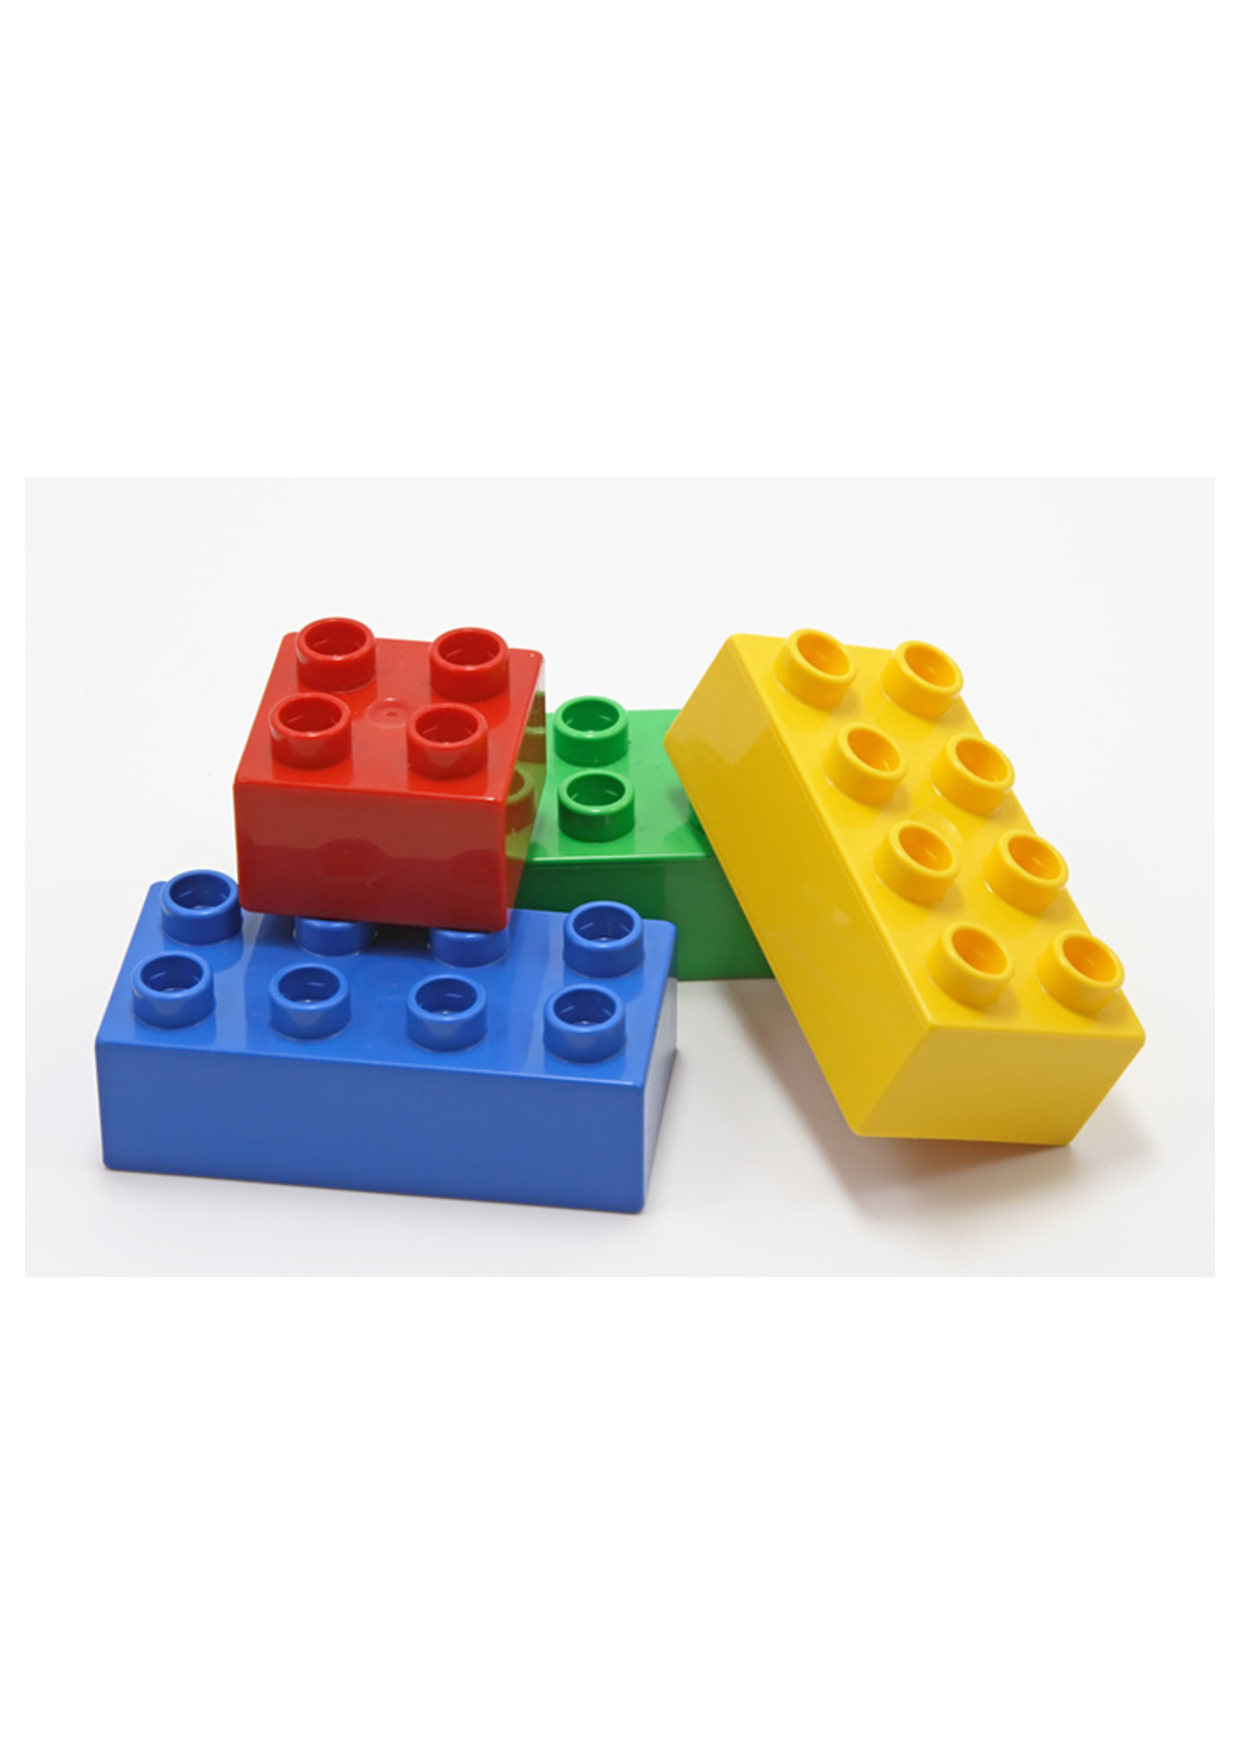
\includegraphics[scale=0.2]{Figures/Signal30.pdf} & \centering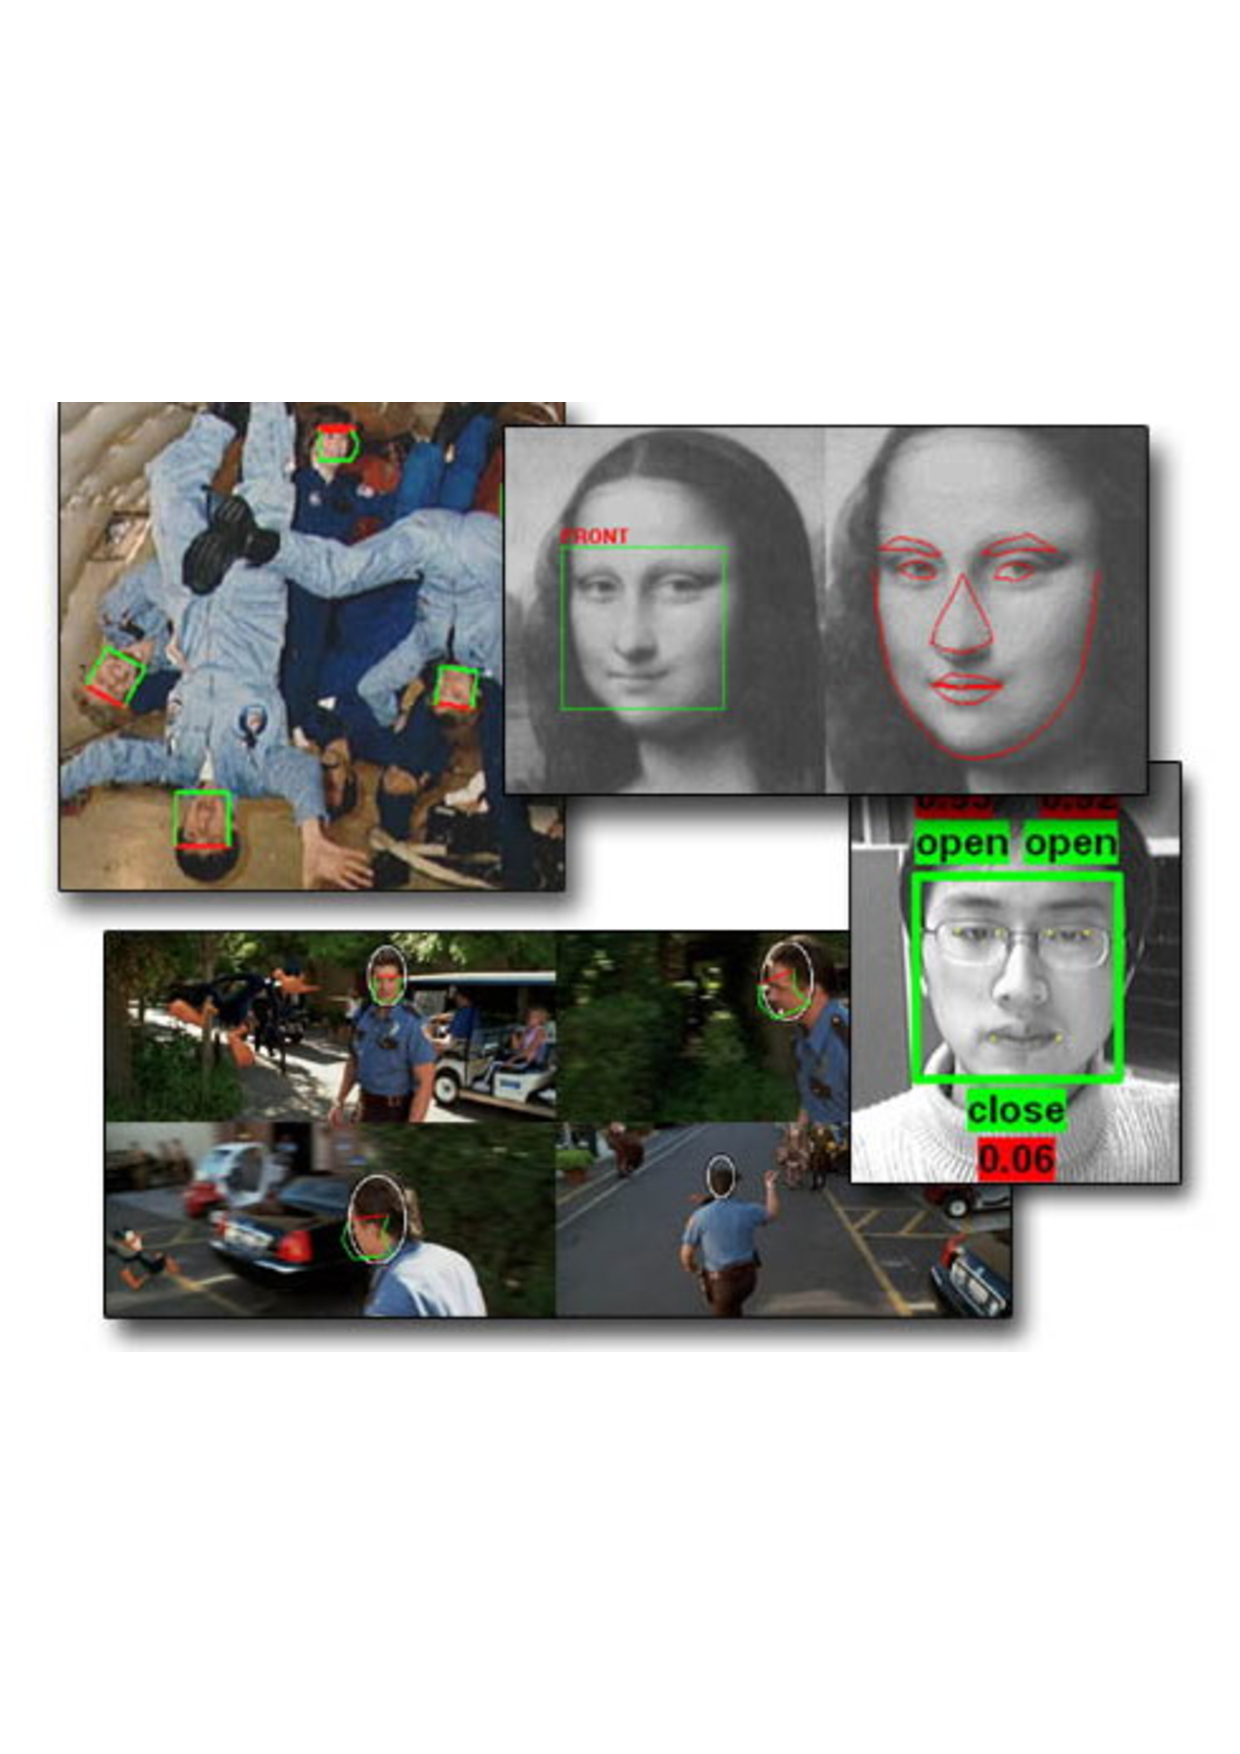
\includegraphics[scale=0.2]{Figures/Signal31.pdf}
\end{tabular}
\begin{figure}
\end{figure}

\begin{alertblock}{}
\textbf{FOUNDATIONS OF ADVANCED SIGNAL PROCESSING.}
\end{alertblock}

}

\frame{
\frametitle{Some cool examples in Pattern Recognition:}

\begin{itemize}
\item Google Vision API: \url{https://cloud.google.com/vision/}
\end{itemize}

\begin{itemize}
\item Object Recognition using Deep Learning: \url{https://www.youtube.com/watch?v=dAl2gimGIpU}
\end{itemize}



\begin{itemize}
\item Simple introduction to Machine Learning: \url{https://medium.com/@ageitgey}
\end{itemize}


}



\end{document}
